\documentclass[t,11pt,aspectratio=169]{beamer}
\usepackage{tikz}
\usepackage{pgfplots}
\usetikzlibrary{calc}
\usepackage[utf8]{inputenc}
\usepackage[ngerman]{babel}
\usepackage{amsmath,amsfonts,amssymb}
\usepackage{framed}
\usecolortheme{orchid}
\usepackage{etoolbox}
\useinnertheme[shadow=true]{rounded}

\usepackage{verbatim}

%%% PROGRESSBAR
\definecolor{pbblue}{HTML}{D8D8D8}% filling color for the progress bar
\definecolor{pbgray}{HTML}{F2F2F2}% background color for the progress bar
\useoutertheme{infolines}
\setbeamerfont{footline}{size=\normalsize}
\setbeamersize{text margin left=30pt,text margin right=30pt}
\makeatletter
\setbeamertemplate{footline}
{
	\leavevmode%
	\hbox{%
		\begin{beamercolorbox}[wd=.333333\paperwidth,ht=2.5ex,dp=1ex,center]{title in head/foot}%
			\usebeamerfont{title in head/foot}\insertshorttitle
		\end{beamercolorbox}%
		\begin{beamercolorbox}[wd=.333333\paperwidth,ht=2.5ex,dp=1ex,center]{date in head/foot}%
			%\usebeamerfont{date in head/foot}\insertshortdate{}\hspace*{2em}
			%\insertframenumber\hspace*{2ex} 
		\end{beamercolorbox}
		\begin{beamercolorbox}[wd=.333333\paperwidth,ht=3ex,dp=1ex,center]{author in head/foot}%
			\usebeamerfont{author in head/foot}\insertshortauthor~~%\beamer@ifempty{\insertshortinstitute}{}{(\insertshortinstitute)}
		\end{beamercolorbox}%
	}%
	\vskip0pt%
}
\makeatother
\makeatletter
\def\progressbar@progressbar{} % the progress bar
\newcount\progressbar@tmpcounta% auxiliary counter
\newcount\progressbar@tmpcountb% auxiliary counter
\newdimen\progressbar@pbht %progressbar height
\newdimen\progressbar@pbwd %progressbar width
\newdimen\progressbar@tmpdim % auxiliary dimension
\progressbar@pbwd=\linewidth
\progressbar@pbht=1.5ex
\def\progressbar@progressbar{%
    \progressbar@tmpcounta=\insertpagenumber
    \progressbar@tmpcountb=\insertdocumentendpage
    \progressbar@tmpdim=\progressbar@pbwd
    \multiply\progressbar@tmpdim by \progressbar@tmpcounta
    \divide\progressbar@tmpdim by \progressbar@tmpcountb
  \begin{tikzpicture}[rounded corners=3pt,very thin]
    \shade[top color=pbgray!20,bottom color=pbgray!20,middle color=pbgray!50]
      (0pt, 0pt) rectangle ++ (\progressbar@pbwd, \progressbar@pbht);
      \shade[draw=pbblue,top color=pbblue!50,bottom color=pbblue!50,middle color=pbblue] %
        (0pt, 0pt) rectangle ++ (\progressbar@tmpdim, \progressbar@pbht);
    \draw[color=normal text.fg!50]  
      (0pt, 0pt) rectangle (\progressbar@pbwd, \progressbar@pbht) 
        node[pos=0.5,color=normal text.fg] {\textnormal{%
             \pgfmathparse{\insertpagenumber*100/\insertdocumentendpage}%
             \pgfmathprintnumber[fixed,precision=0]{\pgfmathresult}\,\%%
        }%
    };
  \end{tikzpicture}%
}
\addtobeamertemplate{headline}{}
{%
  \begin{beamercolorbox}[wd=\paperwidth,ht=4ex,center,dp=1ex]{white}%
    \progressbar@progressbar%
  \end{beamercolorbox}%
}
\makeatother

\setbeamertemplate{frametitle}[default][center]

%%% BLOCKS
% block = Aufgabe
\setbeamercolor{block title}{fg=black,bg=blue!30!white} 
\setbeamercolor{block body}{fg=black, bg=blue!3!white}

% alertblock = Definition
\setbeamercolor{block title alerted}{fg=black,bg=red!50!white} 
\setbeamercolor{block body alerted}{fg=black, bg=red!3!white}

% exampleblock = Wiederholung
\setbeamercolor{block title example}{fg=black,bg=green!30!white} 
\setbeamercolor{block body example}{fg=black, bg=green!3!white}

\setbeamercovered{transparent}
\setbeamertemplate{navigation symbols}{}

\addtocounter{page}{-1}
\addtocounter{framenumber}{-1}
\setbeamercovered{invisible}





\begin{document}

\begin{frame}{Der Kolmogorov-Smirnov-Test}
	\begin{enumerate}
		\item[Fall 1:] Besitzen zwei Zufallsvariablen die gleiche Verteilung? (Zweistichprobenproblem)
		\item[Fall 2:] Folgt eine Zufallsvariable einer bestimmten theoretischen Verteilung? (Einstichprobenproblem, Anpassungstest)
	\end{enumerate}
\end{frame}

\begin{frame}[fragile]
	\begin{enumerate}
		\item[Fall 1:] Besitzen zwei Zufallsvariablen die gleiche Verteilung?
	\end{enumerate}
	Von zwei Zufallsvariablen $X$ und $Y$ liegen die folgenden Stichproben $x$ und $y$ vor:
	\begin{verbatim}
		> x
		-0.9379653 -0.5115044  0.2914135  1.6328312 -1.1932723  
		1.5935587  1.7787011  0.6431912  0.5164562 -1.7528549
		> y
		-0.8204684  0.4874291  0.7383247  0.5757814 -0.3053884  
		1.5117812  0.3898432 -0.6212406 -2.2146999  1.1249309
	\end{verbatim}
	\pause Die Hypothesen lauten:
	\begin{enumerate}
		\item[$H_0$:] $F_X(x) = F_Y(y)$
		\item[$H_1$:] $F_X(x) \neq F_Y(y)$
	\end{enumerate}
\end{frame}

\begin{frame}
\begin{enumerate}
	\item[Fall 1:] Besitzen zwei Zufallsvariablen die gleiche Verteilung?
\end{enumerate}
\begin{center}
	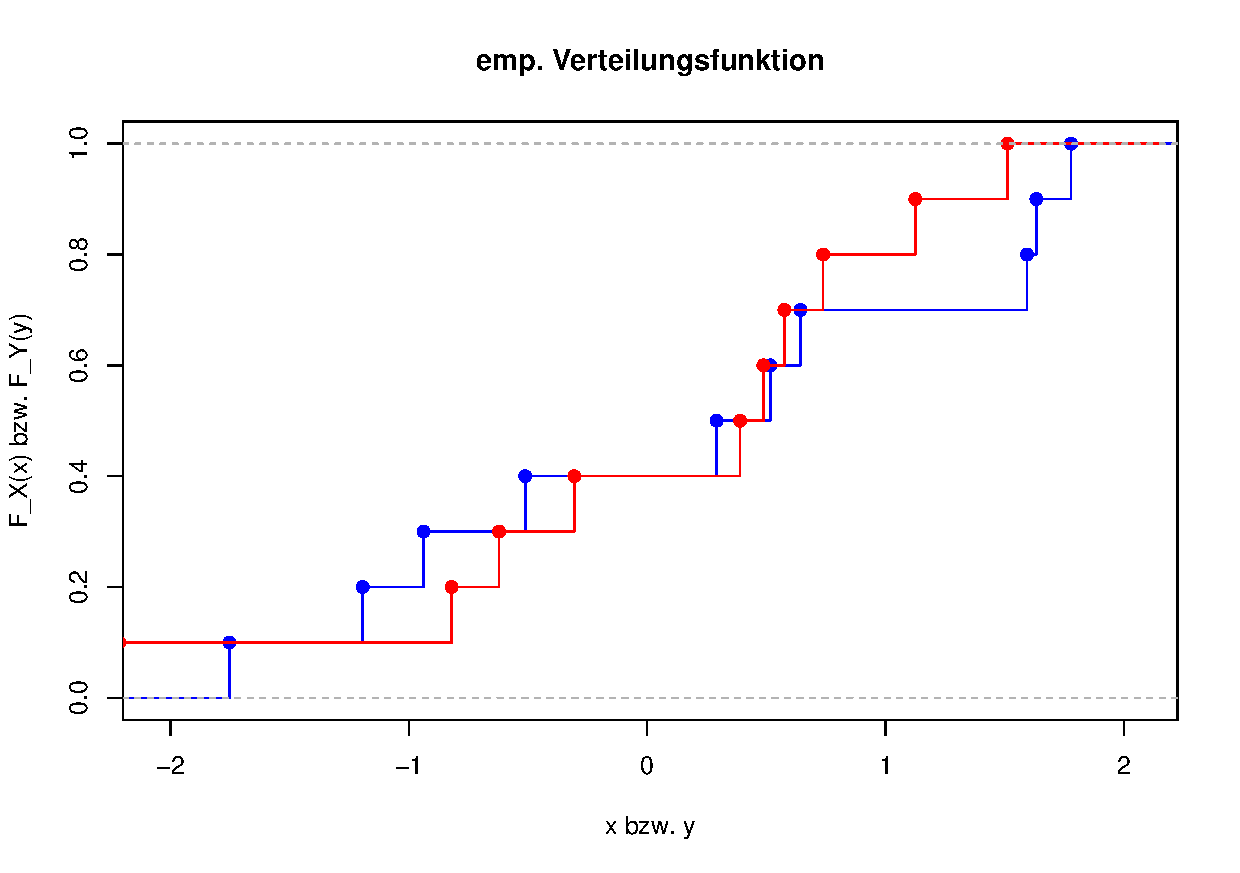
\includegraphics[scale=0.45]{Rplot.pdf}
\end{center}
\end{frame}

\begin{frame}
\begin{enumerate}
	\item[Fall 1:] Besitzen zwei Zufallsvariablen die gleiche Verteilung?
\end{enumerate}
\begin{center}
	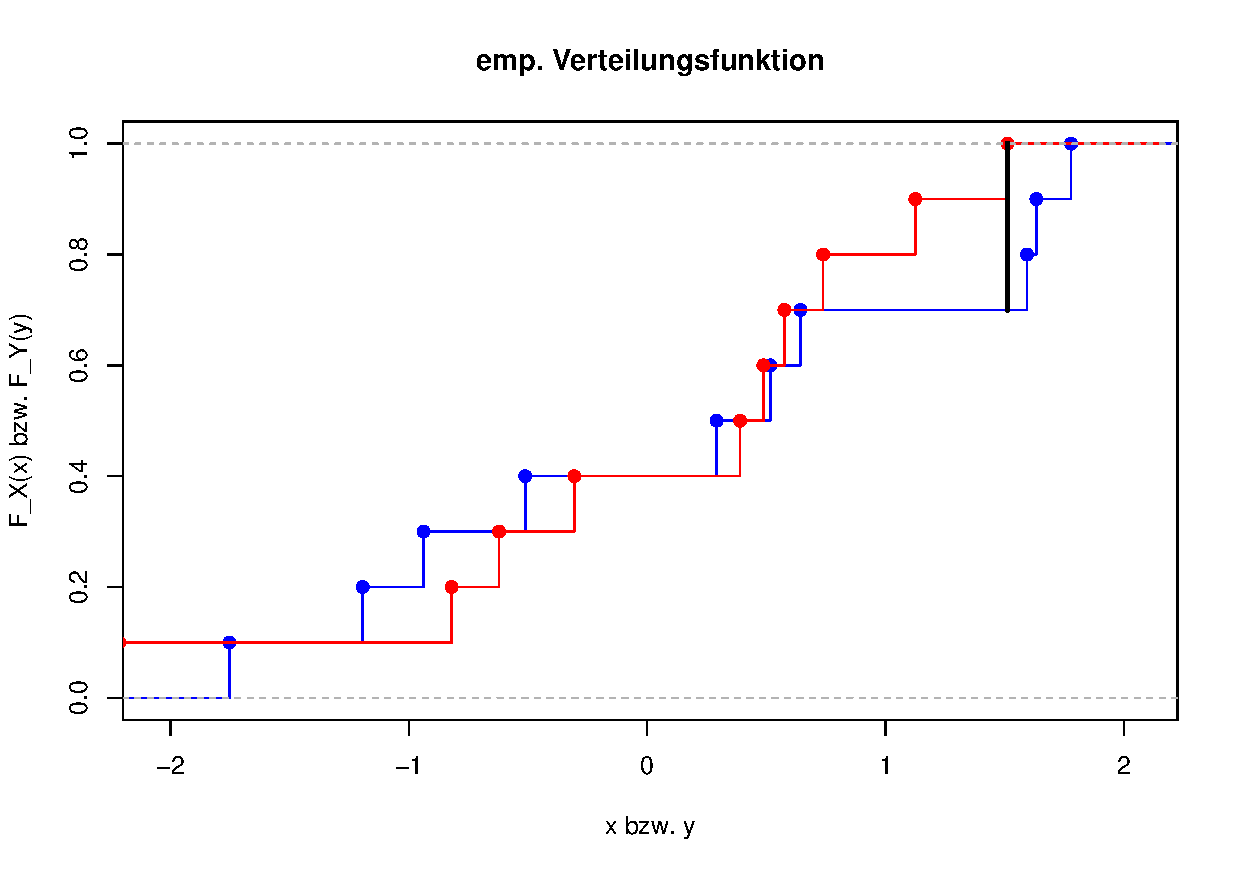
\includegraphics[scale=0.45]{Rplot01.pdf}
\end{center}
\end{frame}

\begin{frame}
\begin{enumerate}
	\item[Fall 1:] Besitzen zwei Zufallsvariablen die gleiche Verteilung?
\end{enumerate}
\begin{center}
	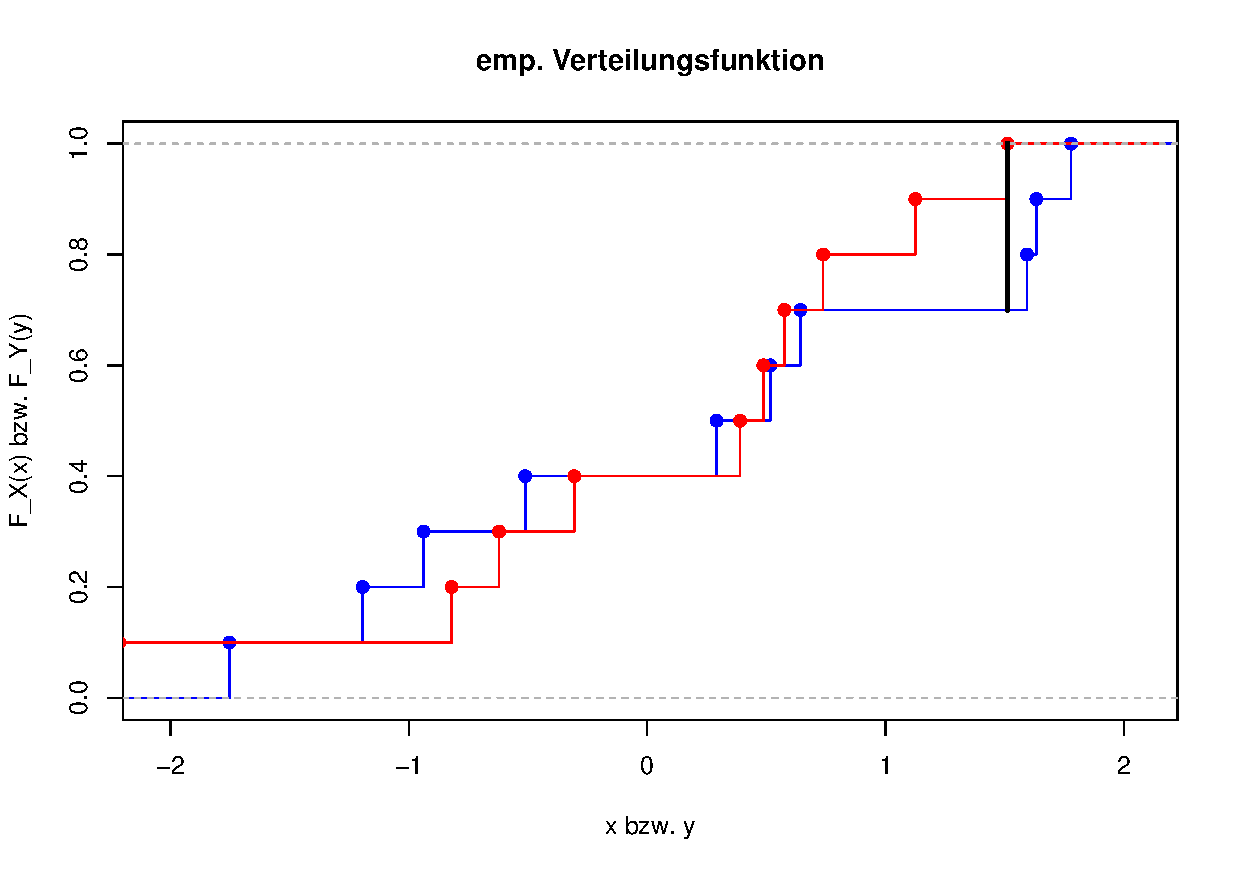
\includegraphics[scale=0.3]{Rplot01.pdf}
\end{center}
\begin{align*}
	d_n = \max \left| F_X(x) - F_Y(y)  \right|,
\end{align*}
wobei $n$ der Stichprobenumfang ist. Übrigens: Die beiden Stichproben müssen nicht den gleichen Stichprobenumfang haben!
\pause
Bei uns ist $d_{10} = 0.3$.
\end{frame}

\begin{frame}[fragile]
	\begin{enumerate}
		\item[Fall 1:] Besitzen zwei Zufallsvariablen die gleiche Verteilung?
	\end{enumerate}
	Die Testentscheidung:
	\begin{enumerate}
		\item Bestimme ein Signifikanzniveau $\alpha$, zum Beispiel $\alpha=5\%$.
		\item Lese den kritischen Wert aus einer Tabelle ab, für $\alpha=5\%$ beträgt dieser $0.7$.
		\item Vergleiche den Wert der Testgröße $d_{10}=0.3$ mit dem kritischen Wert: Da $0.3<0.7$, kann die Nullhypothese $F_X(x)=F_Y(y)$ nicht verworfen werden.
	\end{enumerate}
\pause
	In R:
	\begin{verbatim}
		> ks.test(x,y)
		Two-sample Kolmogorov-Smirnov test
		data:  x and y
		D = 0.3, p-value = 0.7869
	\end{verbatim}
\end{frame}

\begin{frame}[fragile]
	\begin{enumerate}
		\item[Fall 2:] Folgt eine Zufallsvariable einer bestimmten theoretischen Verteilung?
	\end{enumerate}
	\begin{center}
		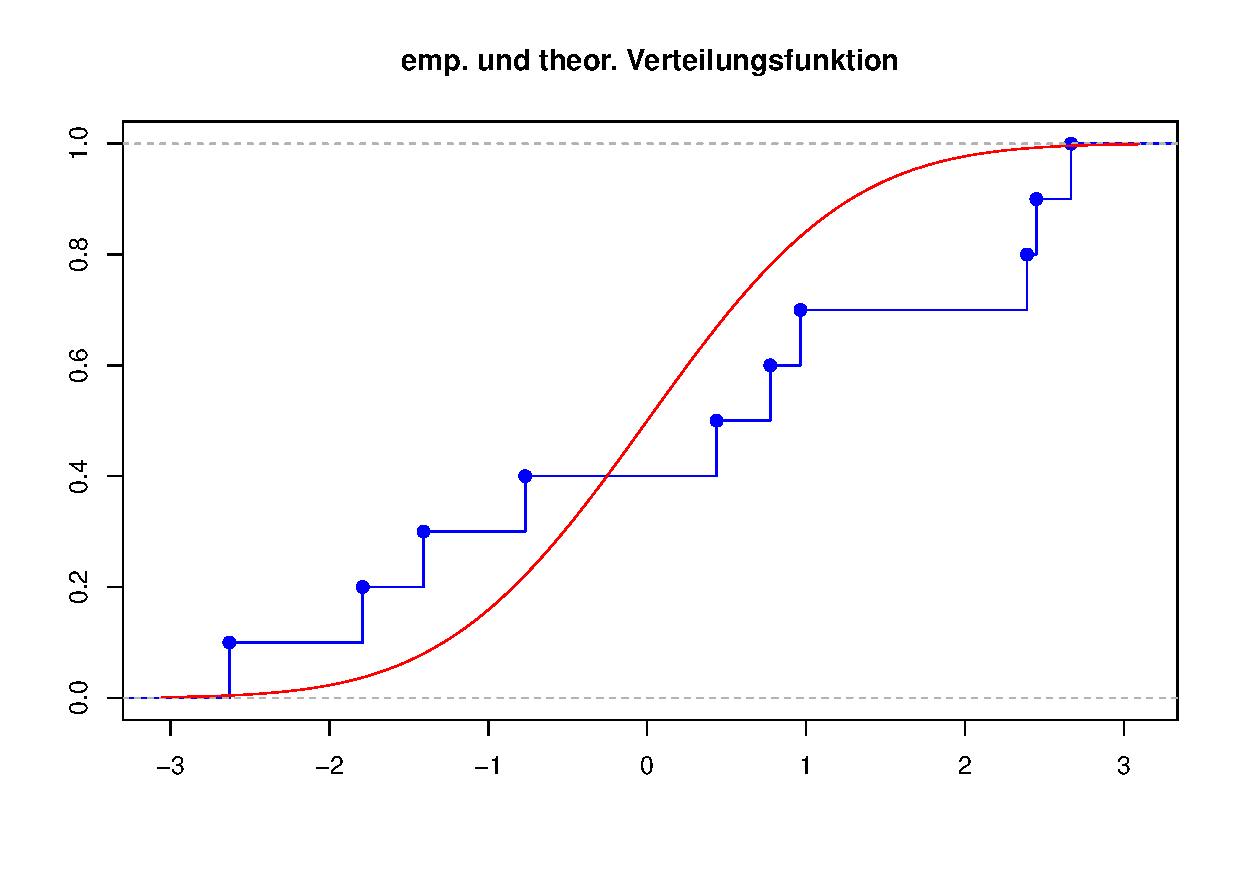
\includegraphics[scale=0.3]{Rplot02.pdf}
	\end{center}
\pause
\begin{verbatim}
> y = runif(10,-3,3); ks.test(y,"pnorm")
One-sample Kolmogorov-Smirnov test
D = 0.29158, p-value = 0.3008
\end{verbatim}
\end{frame}

\begin{frame}[fragile]
\begin{enumerate}
	\item[Fall 2:] Folgt eine Zufallsvariable einer bestimmten theoretischen Verteilung?
\end{enumerate}
\begin{center}
	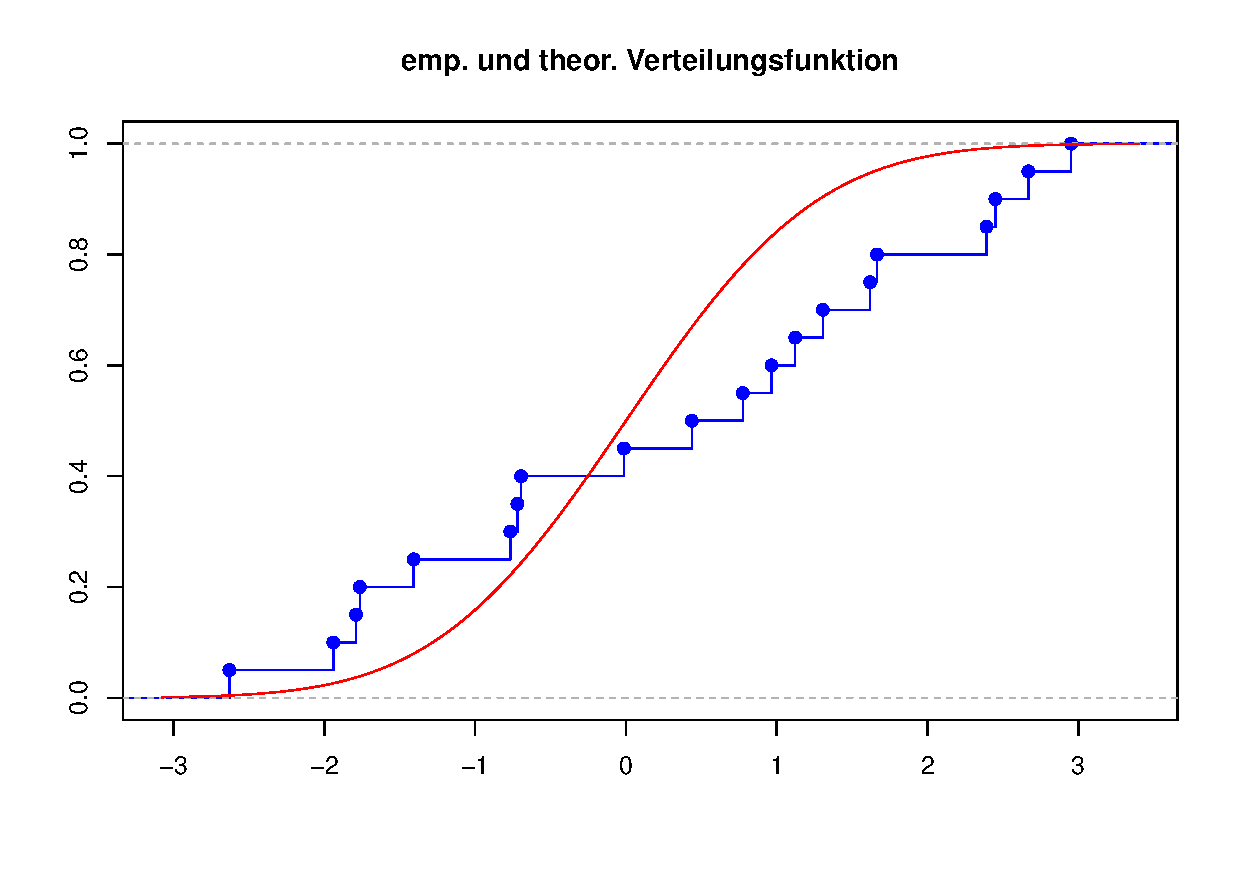
\includegraphics[scale=0.3]{Rplot03.pdf}
\end{center}
\begin{verbatim}
> y = runif(20,-3,3); ks.test(y,"pnorm")
One-sample Kolmogorov-Smirnov test
D = 0.28267, p-value = 0.06605
\end{verbatim}
\end{frame}

\begin{frame}[fragile]
\begin{enumerate}
	\item[Fall 2:] Folgt eine Zufallsvariable einer bestimmten theoretischen Verteilung?
\end{enumerate}
\begin{center}
	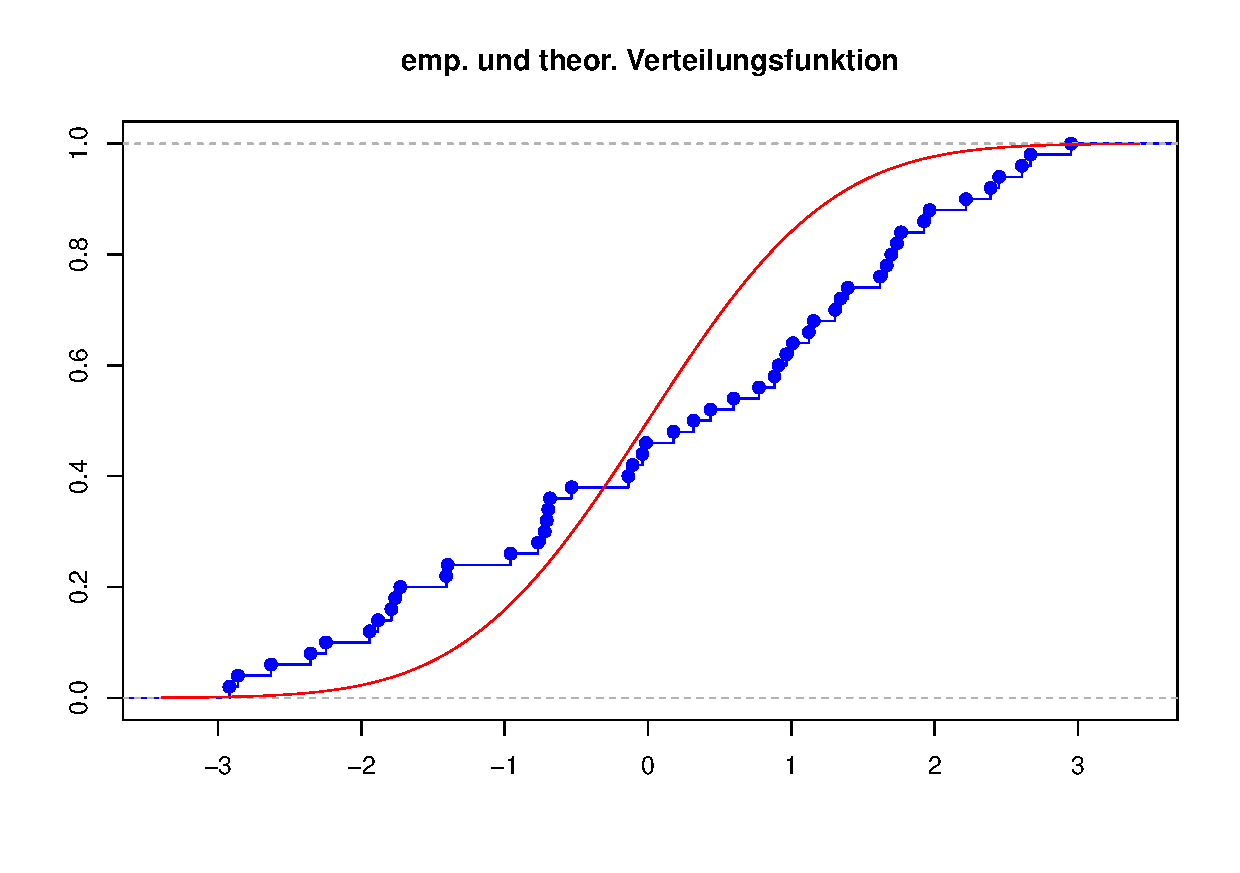
\includegraphics[scale=0.3]{Rplot04.pdf}
\end{center}
\begin{verbatim}
> y = runif(50,-3,3); ks.test(y,"pnorm")
One-sample Kolmogorov-Smirnov test
D = 0.25121, p-value = 0.002879
\end{verbatim}
\end{frame}

\end{document}